\section{Simulation exercises}
Two different simulation exercises are used to compare the
performance of the new compartmental model with that of a
traditional compartmental model. The first simulation exercise
assesses the performance of each type of compartmental model with
respect to an analytical solution of the continuum model. In these
simulations the NEURON simulator (Hines and Carnevale,
\cite{Hines97}) is used to characterise the behaviour of a
traditional compartmental model. The second simulation exercise
compares the behaviour of a traditional compartmental model and
the new compartmental model with respect to the spike train
activity generated in each model by large scale synaptic activity.
In these simulations, a traditional compartmental model developed
by the authors is used. The behaviour of this model in the first
simulation exercise is indistinguishable from that of the NEURON
simulator. Finally, all solutions of the compartmental models are
advanced in one microsecond time steps to ensure that errors in
temporal integration make no significant contribution to the error
in the estimated membrane potential.

\subsection{First simulation exercise}\label{sim1}
The performance of the traditional compartmental model is first
compared against that of the new compartmental model by assessing
the accuracy with which both models determine the time course of
the somal potential of the model neuron (Figure \ref{TestNeuron})
when subjected to large scale exogenous point input. The
comparison relies on the fact that the model neuron has the
property that the effect at its soma of an exogenous input at a
given electrotonic distance from its soma is identical to the
effect at the soma of that input acting on a uniform dendritic
cylinder at the same electrotonic distance from the soma.

Each simulation distributes 75 point inputs at random over the
dendritic tree of the model neuron, where each input has strength
$2\times10^{-5}\,\mu$A. These inputs are then mapped to positions
on the Rall equivalent cylinder at the same electrotonic distance
from the soma (assumed to be a sphere of diameter $40\,\mu$m). The
time course of the potential at the soma of the equivalent
cylinder due to the combined effect of these inputs is determined
analytically and taken to be the reference potential with respect
to which error in both compartmental models is assessed. The
potential at the soma in response to this stimulus regimen is
obtained for the traditional and new compartmental models. The
difference between a computed potential and its exact value is
determined at one millisecond intervals in the first 10
milliseconds of the simulation, and each difference is divided by
the exact potential at that time to get a relative measure of
error at these times. The entire simulation procedure is now
repeated 2000 times for each of 13 different levels of spatial
discretisation (number of compartments).

\subsubsection{Results}
The results for the first simulation exercise of the traditional
and new compartmental models are set out in Table \ref{simex1}.
This table shows the common logarithms of the mean value of the
modulus of the relative error and the standard deviation of that
error estimated at ten milliseconds after the initiation of the
stimulus and based on 2000 simulations for each level of spatial
discretisation (number of compartments). Similar results, not
shown, hold at all time points at which the errors were estimated.

\pagebreak[4]

\begin{table}[!h]
\[
\begin{array}{c|cc|cc}
\hline
\mbox{\begin{tabular}{c} Compartments \\[-5pt]
(log$_{10}(\mbox{Compartments}))$ \end{tabular}} &
\multicolumn{2}{|c|}{\mbox{\begin{tabular}{cc}
NEURON & New Model \\[-5pt] \multicolumn{2}{c}{$\log_{10}$(Mean)}
\end{tabular}}}
& \multicolumn{2}{|c}{\mbox{\begin{tabular}{cc}
NEURON & New Model \\[-5pt] \multicolumn{2}{c}{$\log_{10}$(Standard Dev.)} \end{tabular}}}\\
\hline
\phantom{0}17 \quad (1.2305) & -2.41151 & -2.71945 & -2.62290 & -3.19338 \\
\phantom{0}21 \quad (1.3222) & -2.47233 & -2.77674 & -2.69851 & -3.24583 \\
\phantom{0}34 \quad (1.5314) & -2.94299 & -3.41196 & -3.06731 & -3.88820 \\
\phantom{0}41 \quad (1.6127) & -3.04729 & -3.62138 & -3.17081 & -4.14997 \\
\phantom{0}54 \quad (1.7323) & -3.21258 & -3.89150 & -3.34889 & -4.41251 \\
\phantom{0}61 \quad (1.7853) & -3.24692 & -3.91268 & -3.37653 & -4.45051 \\
\phantom{0}75 \quad (1.8750) & -3.35180 & -4.12056 & -3.46881 & -4.65463 \\
\phantom{0}82 \quad (1.9138) & -3.39846 & -4.23567 & -3.51591 & -4.76498 \\
\phantom{0}93 \quad (1.9684) & -3.45602 & -4.30636 & -3.57633 & -4.82045 \\
          193 \quad (2.2855) & -3.77417 & -4.94731 & -3.89829 & -5.47886 \\
          293 \quad (2.4668) & -3.94409 & -5.31876 & -4.07811 & -5.84771 \\
          390 \quad (2.5910) & -4.08234 & -5.57349 & -4.20025 & -6.10791 \\
          495 \quad (2.6946) & -4.15996 & -5.78252 & -4.28525 & -6.32790 \\
\hline
\end{array}
\]
\centering
\parbox{5in}{\caption{\label{simex1} The results of 2000 simulations
for each of 13 different compartmental models based on the new and
traditional (NEURON) representations of a compartment. The common
logarithms of the mean value of the modulus of the relative error
and the standard deviation of that error are estimated at ten
milliseconds after the initiation of the stimulus.}}
\end{table}

The left hand panel of Figure \ref{mean} shows regression lines of
the common logarithms of the modulus of the mean relative error
for the traditional (dashed line) and new (solid line)
compartmental models on the logarithm of the number of
compartments used to represent the model neuron. These lines are
based on the data in Table \ref{simex1} and have equations
\begin{equation}\label{mean1}
\begin{array}{rcl}
\log_{10}(\mbox{Mean Relative Error: NEURON}) & = &
-1.09-1.17\log_{10}(\mbox{Compartments})\,, \\[5pt]
\log_{10}(\mbox{Mean Relative Error: New Model}) & = &
-0.17-2.10\log_{10}(\mbox{Compartments})
\end{array}
\end{equation}
in which the regressions are achieved with respective adjusted
$R^2$ values of $97.4\%$ and $99.5\%$. In view of their very high
$R^2$ values, a number of conclusions can be drawn from these
results. For a fixed number of compartments, the error in the new
model is always less than that of the traditional model. The
regression equations (\ref{mean1}) support the argument and
subsequent assertion made in Section \ref{assertion} that the
error in a traditional compartmental model is approximately
$O(1/n)$, whereas that in the new compartmental model is
approximately $O(1/n^2)$. In practice, this means that the
accuracy achieved by a traditional compartmental model using
500/100 compartments is achieved in the new compartmental model by
the use of approximately 100/40 compartments.

\begin{figure}[!h]
\centerline{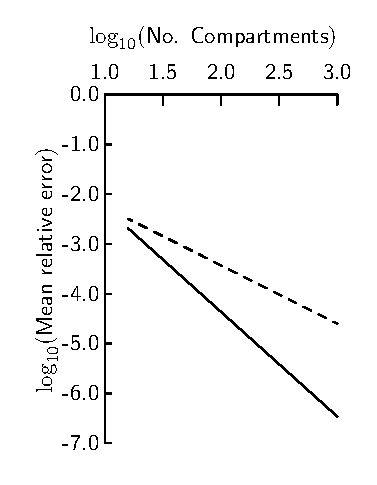
\includegraphics[ ]{NewCompFig5a.eps}
\quad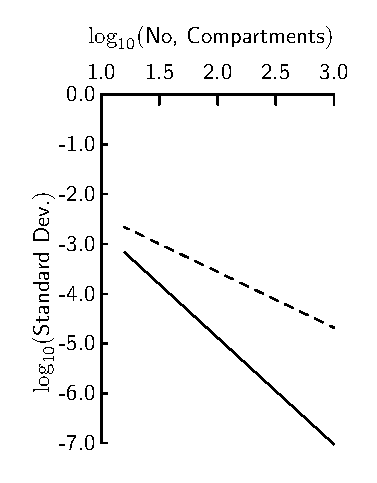
\includegraphics[ ]{NewCompFig5b.eps}}
\centering
\parbox{5.8in}{\caption{\label{mean} The left panel shows the
regression lines of the mean relative errors in the new
compartmental model (solid line) and that of a traditional
compartmental model (NEURON - dashed line) against number of
compartments. All errors are measured ten milliseconds after
initiation of the stimulus. The right panel shows the regression
lines for the standard deviations of the mean relative errors for
the new compartmental model (solid line) and for a traditional
compartmental model (NEURON - dashed line).}}
\end{figure}

%\begin{figure}[!h]
%\centerline{\begin{mfpic}[56][24]{0.4}{3}{-7.5}{1}
%\headlen7pt
%\pen{1pt}
%\dotspace=4pt
%\dotsize=1.5pt
%%
%% x-axis
%\tlabel[br](3.0,0.9){\textsf {$\log_{10}(\mbox{No. Compartments})$}}
%\lines{(1.0,0),(3.0,0)}
%\lines{(1.5,0),(1.5,-0.2)}
%\lines{(2.0,0),(2.0,-0.2)}
%\lines{(2.5,0),(2.5,-0.2)}
%\lines{(3.0,0),(3.0,-0.2)}
%\tlabel[bc](1.0,0.3){\textsf{1.0}}
%\tlabel[bc](1.5,0.3){\textsf{1.5}}
%\tlabel[bc](2.0,0.3){\textsf{2.0}}
%\tlabel[bc](2.5,0.3){\textsf{2.5}}
%\tlabel[bc](3.0,0.3){\textsf{3.0}}
%% y-axis
%\tlabel[bc](0.5,-6){\rotatebox{90}{\textsf{$\log_{10}(\mbox{Mean relative error})$}}}
%\lines{(1,0),(1,-7)}
%\lines{(1.0,-1.0),(1.05,-1.0)}
%\lines{(1.0,-2.0),(1.05,-2.0)}
%\lines{(1.0,-3.0),(1.05,-3.0)}
%\lines{(1.0,-4.0),(1.05,-4.0)}
%\lines{(1.0,-5.0),(1.05,-5.0)}
%\lines{(1.0,-6.0),(1.05,-6.0)}
%\lines{(1.0,-7.0),(1.05,-7.0)}
%\tlabel[cr](0.95,-0.0){\textsf{0.0}}
%\tlabel[cr](0.95,-1.0){\textsf{-1.0}}
%\tlabel[cr](0.95,-2.0){\textsf{-2.0}}
%\tlabel[cr](0.95,-3.0){\textsf{-3.0}}
%\tlabel[cr](0.95,-4.0){\textsf{-4.0}}
%\tlabel[cr](0.95,-5.0){\textsf{-5.0}}
%\tlabel[cr](0.95,-6.0){\textsf{-6.0}}
%\tlabel[cr](0.95,-7.0){\textsf{-7.0}}
%%
%% Mean values at t=10
%\dashed\lines{(1.2,-2.494),(3.0,-4.60)}
%\lines{(1.2,-2.686),(3.0,-6.466)}
%\end{mfpic}
%\begin{mfpic}[56][24]{0}{3}{-7.5}{1}
%\headlen7pt
%\pen{1pt}
%\dotspace=4pt
%\dotsize=1.5pt
%%
%% x-axis
%\tlabel[br](3.0,0.9){\textsf{$\log_{10}(\mbox{No, Compartments})$}}
%\lines{(1.0,0),(3.0,0)}
%\lines{(1.5,0),(1.5,-0.2)}
%\lines{(2.0,0),(2.0,-0.2)}
%\lines{(2.5,0),(2.5,-0.2)}
%\lines{(3.0,0),(3.0,-0.2)}
%\tlabel[bc](1.0,0.3){\textsf{1.0}}
%\tlabel[bc](1.5,0.3){\textsf{1.5}}
%\tlabel[bc](2.0,0.3){\textsf{2.0}}
%\tlabel[bc](2.5,0.3){\textsf{2.5}}
%\tlabel[bc](3.0,0.3){\textsf{3.0}}
%% y-axis
%\tlabel[bc](0.5,-6){\rotatebox{90}{\textsf{$\log_{10}(\mbox{Standard Dev.})$}}}
%\lines{(1,0),(1,-7)}
%\lines{(1.0,-1.0),(1.05,-1.0)}
%\lines{(1.0,-2.0),(1.05,-2.0)}
%\lines{(1.0,-3.0),(1.05,-3.0)}
%\lines{(1.0,-4.0),(1.05,-4.0)}
%\lines{(1.0,-5.0),(1.05,-5.0)}
%\lines{(1.0,-6.0),(1.05,-6.0)}
%\lines{(1.0,-7.0),(1.05,-7.0)}
%\tlabel[cr](0.95,-0.0){\textsf{0.0}}
%\tlabel[cr](0.95,-1.0){\textsf{-1.0}}
%\tlabel[cr](0.95,-2.0){\textsf{-2.0}}
%\tlabel[cr](0.95,-3.0){\textsf{-3.0}}
%\tlabel[cr](0.95,-4.0){\textsf{-4.0}}
%\tlabel[cr](0.95,-5.0){\textsf{-5.0}}
%\tlabel[cr](0.95,-6.0){\textsf{-6.0}}
%\tlabel[cr](0.95,-7.0){\textsf{-7.0}}
%%
%% Standard deviations at t=10
%\dashed\lines{(1.2,-2.664),(3.0,-4.680)}
%\lines{(1.2,-3.169),(3.0,-7.021)}
%\end{mfpic}}
%\centering
%\parbox{5.8in}{\caption{\label{mean} The left panel shows the
%regression lines of the mean relative errors in the new
%compartmental model (solid line) and that of a traditional
%compartmental model (NEURON - dashed line) against number of
%compartments. All errors are measured ten milliseconds after
%initiation of the stimulus. The right panel shows the regression
%lines for the standard deviations of the mean relative errors for
%the new compartmental model (solid line) and for a traditional
%compartmental model (NEURON - dashed line).}}
%\end{figure}

\pagebreak[4]

The standard deviation (SD) of the modulus of the relative error
can be regarded as an indicator of the reliability of a single
application of the model. The right hand panel of Figure
\ref{mean} shows regression lines of the common logarithms of the
standard deviation of the modulus of the relative error for the
traditional (dashed line) and new (solid line) compartmental
models on the logarithm of the number of compartments used to
represent the model neuron. These lines are based on the data in
Table \ref{simex1} and have equations
\begin{equation}\label{mean1}
\begin{array}{rcl}
\log_{10}(\mbox{SD of Relative Error: NEURON}) & = &
-1.32-1.12\log_{10}(\mbox{Compartments})\,, \\[5pt]
\log_{10}(\mbox{SD of Relative Error: New Model}) & = &
-0.60-2.14\log_{10}(\mbox{Compartments})
\end{array}
\end{equation}
in which the regressions are achieved with respective adjusted
$R^2$ values of $98.7\%$ and $99.4\%$. These lines show that the
new compartmental model is more reliable than a traditional
compartmental model. For example, a traditional compartmental
model requires at least 100 compartments to give a standard
deviation of the modulus of the relative error that is smaller
than that of the new compartmental model using 40 compartments.

\subsection{Second simulation exercise}\label{sim2}

In the second simulation exercise 100 synapses are distributed at
random over the dendritic tree of the model neuron illustrated in
Figure \ref{TestNeuron}. Each synapse is activated independently
of all other synapses, has a maximum conductance of
$3\times10^{-5}\,\mbox{mS}$ and a time constant of $0.5$ msec.
Activation times for each synapse follow Poisson statistics with a
mean rate of 30 pre-synaptic spikes per second. By contrast with
the first simulation exercise in which the somal membrane was
passive, the behaviour of the somal membrane in the second
simulation exercise is active and obeys Hodgkin-Huxley kinetics.
This simulation exercise is based on 12 different levels of
spatial discretisation (number of compartments) in which each
simulation of the traditional and new compartmental models use
identical synaptic firing times and identical numbers of
compartments.

\subsubsection{Results}
Table \ref{spikerate} gives the spike rate of soma-generated
action potentials based on 11 seconds of activity, the first
second of which is ignored.

\begin{table}[!h]
\[
\begin{array}{c|c|c}
\hline
\mbox{\begin{tabular}{c}
Compartments \\[-5pt] (log$_{10}(\mbox{Compartments}))$
\end{tabular}} &
\mbox{\begin{tabular}{c}
Traditional Model \\[-5pt] Mean Firing Rate
\end{tabular}}
&\mbox{\begin{tabular}{c}
New Model \\[-5pt] Mean Firing Rate \end{tabular}}\\
\hline
\phantom{0}34 \quad (1.5314) & 31.5 & 27.6 \\
\phantom{0}41 \quad (1.6127) & 30.3 & 27.9 \\
\phantom{0}54 \quad (1.7323) & 30.5 & 27.5 \\
\phantom{0}61 \quad (1.7853) & 29.8 & 27.2 \\
\phantom{0}75 \quad (1.8750) & 29.2 & 27.0 \\
\phantom{0}82 \quad (1.9138) & 28.5 & 27.0 \\
\phantom{0}93 \quad (1.9684) & 28.3 & 26.8 \\
          193 \quad (2.2855) & 26.5 & 26.5 \\
          293 \quad (2.4668) & 25.9 & 26.2 \\
          390 \quad (2.5910) & 26.2 & 26.2 \\
          495 \quad (2.6946) & 26.7 & 26.2 \\
          992 \quad (2.9965) & 26.0 & 26.1 \\
\hline
\end{array}
\]
\centering
\parbox{5in}{\caption{\label{simex2} The results of the second
simulation exercise for a traditional compartmental model and the
new compartmental model in which 10 second records of spike train
activity are obtained for both models for 12 different levels of
spatial discretisation (number of compartments).}}
\end{table}

Figure \ref{spikerate} illustrates the data set out in Table
\ref{simex2} in which the spike rates for the traditional model
(dashed line) and new model (solid line) are plotted against the
common logarithm of the number of compartments used in each
simulation. As the number of compartments used in each model is
increased, the spike rates generated by both models approach a
common limit. However, the spike rate of the traditional model
oscillates about this limit whereas that for the new model
approaches the limit in a monotonic fashion, and achieves the
limiting value with fewer compartments. For example, the spike
rate obtained using the traditional model with 100 compartments is
achieved with only 40 compartments in the new model. The spike
rate obtained using the traditional model with 500 compartments is
achieved in the new model with only 100 compartments. These
differences in the number of compartments required to achieve the
same level of accuracy in both models are identical to those
observed in the first simulation exercise.

\begin{figure}[!h]
\centering
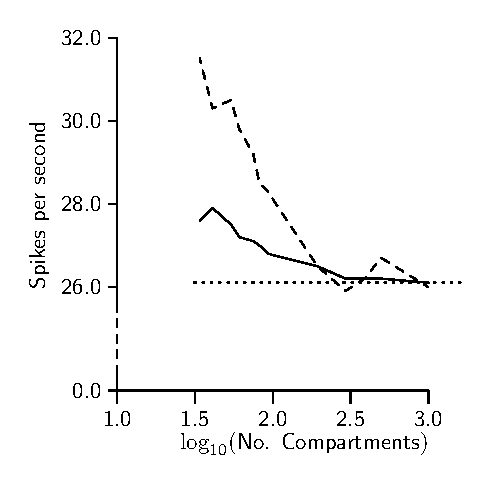
\includegraphics[ ]{NewCompFig6.eps}
\vskip5pt
\parbox{5.5in}{\caption{\label{spikerate} The spike rate plotted against
the common logarithm of the number of compartments for a
traditional compartmental model (dashed line) and the new
compartmental model (solid line). The dotted line shows the
expected spike rate.}}
\end{figure}

%\begin{figure}[!h]
%\centerline{\begin{mfpic}[75][20]{0.3}{3}{-1}{8.5}
%\headlen7pt
%\pen{1pt}
%\dotspace=4pt
%\dotsize=1.5pt
%%
%% x-axis
%\tlabel[tr](3.0,-1){\textsf {$\log_{10}(\mbox{No. Compartments})$}}
%\lines{(1.0,0),(3.0,0.0)}
%\lines{(1.0,0),(1.0,-0.3)}
%\lines{(1.5,0),(1.5,-0.3)}
%\lines{(2.0,0),(2.0,-0.3)}
%\lines{(2.5,0),(2.5,-0.3)}
%\lines{(3.0,0),(3.0,-0.3)}
%\tlabel[tc](1.0,-0.5){\textsf{1.0}}
%\tlabel[tc](1.5,-0.5){\textsf{1.5}}
%\tlabel[tc](2.0,-0.5){\textsf{2.0}}
%\tlabel[tc](2.5,-0.5){\textsf{2.5}}
%\tlabel[tc](3.0,-0.5){\textsf{3.0}}
%%
%% Expected spike rate
%\dotted\lines{(1.5,2.6),(3.2,2.6)}
%%
%% Traditional model (Modulo spike rate of 25)
%\dashed\lines{
%(1.531,8.0),(1.613,6.8),(1.732,7.0),(1.785,6.3),
%(1.875,5.7),(1.914,5.0),(1.968,4.8),(2.286,3.0),
%(2.467,2.4),(2.591,2.7),(2.696,3.2),(2.997,2.5)}
%%
%% New model (Modulo spike rate of 25)
%\lines{
%(1.531,4.1),(1.613,4.4),(1.732,4.0),(1.785,3.7),
%(1.875,3.6),(1.914,3.5),(1.968,3.3),(2.286,3.0),
%(2.467,2.7),(2.591,2.7),(2.695,2.7),(3.000,2.6)}
%% y-axis
%\lines{(1,0),(1,0.5)}
%\dashed\lines{(1,0.5),(1,2.0)}
%\lines{(1,2.0),(1,8.5)}
%\lines{(1.0,0.0),(0.95,0.0)}
%\lines{(1.0,2.5),(0.95,2.5)}
%\lines{(1.0,4.5),(0.95,4.5)}
%\lines{(1.0,6.5),(0.95,6.5)}
%\lines{(1.0,8.5),(0.95,8.5)}
%\tlabel[cr](0.9,0.0){\textsf{0.0}}
%\tlabel[cr](0.9,2.5){\textsf{26.0}}
%\tlabel[cr](0.9,4.5){\textsf{28.0}}
%\tlabel[cr](0.9,6.5){\textsf{30.0}}
%\tlabel[cr](0.9,8.5){\textsf{32.0}}
%\tlabel[tc](0.5,6.5){\rotatebox{90}{\textsf{Spikes per second}}}
%\end{mfpic}}
%\centering
%\vskip5pt
%\parbox{5.5in}{\caption{\label{spikerate} The spike rate plotted against
%the common logarithm of the number of compartments for a
%traditional compartmental model (dashed line) and the new
%compartmental model (solid line). The dotted line shows the
%expected spike rate.}}
%\end{figure}

\section{Concluding remarks}
This investigation has demonstrated that it is possible to achieve
a significant increase in the accuracy and precision of
compartmental models once the actual placement of input is
reflected in the structure of the compartmental model. This
finding is relevant to recent physiological studies that have
demonstrated the extreme accuracy of the timing of events in spike
trains (\emph{e.g.}, Fellous \emph{et al}., \cite{Fellous01}). To
investigate this phenomenon it is essential that the numerical
solution of the mathematical model accounting for this behaviour
is sufficiently accurate to allow one to distinguish between
different biophysical models. The simulation exercises demonstrate
that the new compartmental model is better able to achieve this
aim than a traditional compartmental model using an identical
number of compartments.

\section*{Acknowledgement}
A.E. Lindsay would like to thank the Wellcome Trust for the award
of Vacation Scholarship (VS/03/GLA/8/SL/TH/FH).
